% !TeX root = ../full_report.tex

% TODO possibly images showing saliency map/feature map of filter
% before and after fine-tuning

\chapter{Contributions}
In the last chapter, we have presented the state of the art and related work in
image classification as well as image retrieval, and their limitations when
applied to the instance search problem.
In order to overcome these limitations, we proceed as follows.

We first look at the instance retrieval problem as a
classification problem, with each instance representing a class.
We use transfer learning in order to fine-tune
a deep CNN pre-trained on ImageNet to this new task. This approach
is detailed in Section~\ref{sec:finetuning}.

We then consider the instance retrieval problem as an image retrieval
problem. We simplify the state-of-the-art architecture by removing
region of interest pooling and apply this simplified Siamese architecture
to our research problem. This approach can be seen as fine-tuning a network
on image matching. This is detailed in Section~\ref{sec:simplifiedsiam}.

In Section~\ref{sec:analysisprev}, we identify the limitations of the
state of the art as well as the network fine-tuned on classification
in more detail. We also show that good region descriptors can be obtained
directly from a network fine-tuned on classification.

Based on the observations and analysis from Section~\ref{sec:analysisprev},
we propose a novel approach, which combines fine-tuning a network on
classification and fine-tuning it on image matching using a Siamese
architecture. This approach is presented in Section~\ref{sec:proposed}.

Finally, in Section~\ref{sec:improvedesc} we discuss additional
improvements for descriptors used in image retrieval and propose
an adaption of database feature augmentation to the instance retrieval problem.

\section{Fine-tuning a CNN}\label{sec:finetuning}
In image classification using deep CNNs, we rely on large amounts of data, with high inter-class variability in order to infer the optimal values for
millions of parameters. These parameters allow the CNN to describe the
patterns that an image consists of, from the lowest abstraction layer to
the highest. In the instance search problem, as we want to identify a particular instance, the variability of examples of that instance is less important. This means the data is usually not sufficient to fully optimize a network like ResNet.

In order to overcome this problem, a first possible approach is to fine-tune
a classification network to instance classification. This means that
we consider each instance as a class, and optimize using a cross-entropy
loss, typical for classification.

\begin{equation}\label{eq:crossent}
\mathcal{L} = \frac{1}{N}
\sum_{i=1}^N -y_i \log \hat{y}_i - (1-y_i) \log (1-\hat{y}_i)
= \frac{1}{N} \sum_{i=1}^N \mathit{CE}_i
\end{equation}

Equation~\ref{eq:crossent} describes the cross-entropy loss for a
given instance. $N$ is the number of samples, $y_i$ an indicator
variable taking the value $1$ if sample $i$ belongs to the given
instance and $0$ otherwise, and $\hat{y}_i$ is the predicted probability
that sample $i$ belongs to the given instance. In the following,
we denote the cross-entropy loss for the $i$-th sample as
$\mathit{CE}_i$.

Fine-tuning a CNN for classification on different data has been studied
intensively by Yosinki et al.~\cite{yosinski_how_2014}. In particular,
their study shows that it is only important to fine-tune the neurons
of higher layers of a CNN. Furthermore, they show that
fine-tuning can increase generalization even in the fine-tuned model.
Both of these properties are desirable in our task, because they reduce
the memory and time needed to re-train a network, as well as the need
for a large dataset used for fine-tuning.

The specific considerations we take with regards to fine-tuning are
described in the following sections.

\subsection{Data augmentation}
Our datasets, presented in Section~\ref{sec:datasets},
contain an average of less than 10 samples per instance.
This makes training a typical CNN model difficult,
even when fine-tuning for classification.
Data augmentation consists of randomly applying
affine transformations, color perturbations and other random transformations.
It can help in obtaining a more robust network, with higher
geometry invariance than if the network is trained without data
augmentation.
% TODO possibly reference some paper here

Since we specifically identified an issue related to different scales
in images in Section~\ref{sec:limitations} and Section~\ref{sec:incorrectimages},
it is natural to augment the data by randomly scaling the images in both
dimensions.

The lack of geometry invariance of the model can also be reduced by
randomly rotating and flipping the images,
thus we perform this type of data augmentation
throughout our experiments.

For data augmentation in order to fine-tune a CNN, we use the
following values in our experiments:
\begin{enumerate}
    \item Rotation: any angle is chosen with the same probability.
    \item Scaling: the scaling factor is chosen independently for each
    dimension in the range $[0.75,1.25]$.
    \item Flipping: with probability $0.5$, images are horizontally
    flipped.
\end{enumerate}

\subsection{Transfer learning}
The modularity of a CNN means that we can easily transfer
the weights from a pre-trained model, and only re-train the highest
abstraction layers. Specifically, we re-train all linear layers in the
model, representing the highest-level layers.

We also re-train the highest level convolutional layers, since our datasets
contain many visually different images as compared to the ImageNet
dataset used for pre-training the models.
For the AlexNet architecture, we choose to re-train all layers above
and including the last convolutional layer.
For a ResNet architecture, we re-train all layers above and including the
third to last block of convolutional layers. This contains the
nine highest convolutional layers in total.

The results obtained by transfer learning are listed in Table~\ref{tab:results} in chapter~\ref{chap:results}, abbreviated by \emph{FT}.

\section{Simplified Siamese architecture}\label{sec:simplifiedsiam}
We propose a simplified Siamese architecture inspired by the methodology
of Gordo et al.~\cite{gordo_deep_2016}. As shown in
Figure~\ref{fig:gordo_train}, the previous state of the art is set
by a Siamese architecture using the triplet loss.

\subsection{Triplet loss}\label{sec:tripletloss}
\begin{equation}\label{eq:tripletloss}
\mathcal{L} = \sum_{i=1}^N \frac{1}{2}
\max(0, \|x^a_i - x^p_i\|_2^2 - \|x^a_i - x^n_i\|_2^2 + 2m)
\end{equation}

Equation~\ref{eq:tripletloss} describes the triplet loss for $N$
triplets. Each triplet is composed of an anchor image with descriptor
$x^a$, a positive/relevant image with descriptor $x^p$ and a
negative/non-relevant image with descriptor $x^n$. A margin $m$ is added
to the loss, which describes the distance at which two images are
considered similar enough to be relevant with respect to each other.
Throughout our experiments, this margin is set to a value of $m=0.1$.

In image retrieval, many approaches use $l2$-normalized descriptors
~\cite{jegou_hamming_2008,jegou_aggregating_2010,tolias_particular_2015,gordo_deep_2016} since this improves performance and facilitates comparison
between two descriptors. We choose to use $l2$-normalization as well,
which enables us to re-write the triplet loss.

For normalized descriptors $x$ and $y$, the squared distance $\| x - y \|_2^2$
is closely related to the cosine similarity and the dot product through
the relationship derived in Equation~\ref{eq:sqdistcosdot}. One consequence
of this equation is that comparing descriptors based on dot product,
cosine similarity and squared distance is closely related: a high value
of the dot product, high value of cosine similarity and a low value of
the squared distance are all equivalent up to a constant factor and
constant shift.

\begin{equation}\label{eq:sqdistcosdot}
\begin{array}{ll}
\multicolumn{2}{l}{\forall x, y \in \mathbb{R}^n, \|x\|_2 = 1, \|y\|_2 = 1}\\
\|x-y\|_2^2 &= (x_1-y_1)^2 + \dots + (x_n-y_n)^2\\
&=(x_1^2 + \dots + x_n^2) - 2(x_1y_1 + \dots + x_ny_n) +
(y_1^2 + \dots + y_n^2)\\
&=2 - 2xy = 2 - 2\cos(x, y)
\end{array}
\end{equation}

Another consequence of Equation~\ref{eq:sqdistcosdot} is that we can re-write the triplet loss using the dot product, as shown in Equation~\ref{eq:tripletlossnorm}.
This equation represents the version of the triplet loss used in
our experiments. This means all descriptors must be $l2$-normalized before
the loss is evaluated.

\begin{equation}\label{eq:tripletlossnorm}
\mathcal{L} = \sum_{i=1}^N
\max(0, x^a_i x^n_i - x^a_i x^p_i + m)
\end{equation}

\subsection{Simplified architecture}
We simplify the architecture shown in Figure~\ref{fig:gordo_train}
by removing the region proposal network and region of interest pooling.
We justify in Section~\ref{sec:roi} why these components are not
relevant for our datasets and research problem in general.
Except for this change, the architecture is kept exactly as described
by Figures~\ref{fig:gordo_deploy}~and~\ref{fig:gordo_train}.

Just as suggested by previous authors
~\cite{gordo_deep_2016,schroff_facenet:_2015}, when training the Siamese
model, it is initialized with weights of a model fine-tuned on classification
on the same dataset. Here, this fine-tuning is performed as described in
Section~\ref{sec:finetuning} above.

\subsection{Triplet selection}~\label{sec:tripletselection}
As noted by previous authors, when using the triplet loss, it is
crucial to choose the best triplets during training in order to
obtain convergence. In particular, many triplets are irrelevant
and do not produce any loss since they are \emph{too easy} for the network.

Hence, the first idea is to choose the hardest triplets, as proposed by
Schroff et al.~\cite{schroff_facenet:_2015}. However, as they show in
their paper, this can lead to a collapsing model early on in training
so they choose \emph{semi-hard} triplets instead. Semi-hard triplets
are obtained as follows:
use all possible positive couples of images: couples of images from the
same instance. For each positive couple, choose the hardest negative
that is easier than the positive couple. Hard and easy are defined
by the dot product between the descriptors of the images: a high value
of the dot product for images of the same instance represents an easy
positive couple, a high value of the dot product for images of different
instances represents a hard negative couple.
The value of all dot products are determined before each pass over
the whole training data during training, for all couples of images.

A different triplet selection mechanism was proposed by
Gordo et al.~\cite{gordo_end--end_2017}.
First, calculate the values of dot products for all couples of
images before each pass over the training data, as in the method described
above.
Second, for each image, choose the $n$ easiest positive images and the
$m$ hardest negatives. Then, calculate the loss for all possible combinations
and use the $o$ triplets with the highest loss.
This method probably eliminates some noise when choosing the easiest
positive couples, for images that are labeled as being the same instance
but are not visually similar.
However, in experiments, we found that this method does not perform well
for datasets with few images per instance, since we either have to
choose $n$ as very low or we end up choosing all positive couples for
most instances, just like in the \emph{semi-hard} selection.

Hence, in our experiments, we choose the semi-hard triplet selection
for the first two passes over the dataset, after which we only choose
the hardest negatives for all positive couples.

The results obtained by this simplified Siamese architecture, using semi-hard
triplet selection, are listed in Table~\ref{tab:results} in chapter~\ref{chap:results}, abbreviated by \emph{SS}.

\section{Region of interests and object localization}\label{sec:analysisprev}
\subsection{Identifying regions of interest}\label{sec:roi}
\begin{figure}
\centering
\begin{subfigure}[b]{0.3\textwidth}
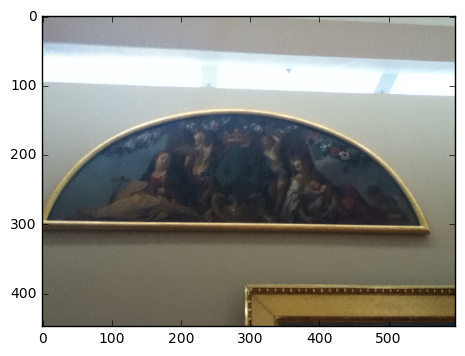
\includegraphics[width=\textwidth]{img/sample1_10A-0519.png}
\caption{Image with label 10A\label{fig:sample1_id}}
\end{subfigure}
\begin{subfigure}[b]{0.3\textwidth}
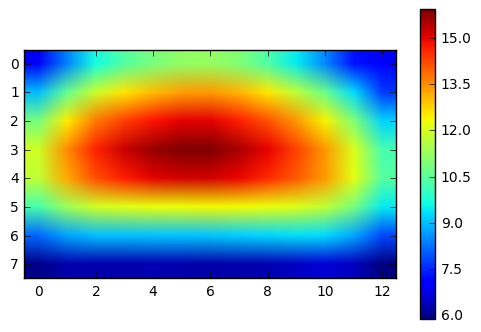
\includegraphics[width=\textwidth]{img/sample1_heatmap.png}
\caption{Heat-map for 10A\label{fig:sample1_hm}}
\end{subfigure}
\begin{subfigure}[b]{0.3\textwidth}
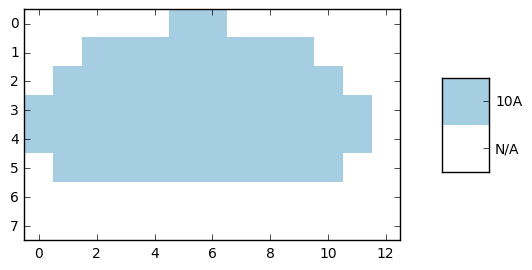
\includegraphics[width=\textwidth]{img/sample1_labels.png}
\caption{Label-map for 10A\label{fig:sample1_lab}}
\end{subfigure}

\begin{subfigure}[b]{0.3\textwidth}
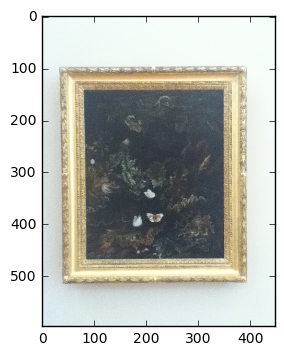
\includegraphics[width=\textwidth]{img/sample2_5P-0508.png}
\caption{Image with label 5P\label{fig:sample2_id}}
\end{subfigure}
\begin{subfigure}[b]{0.3\textwidth}
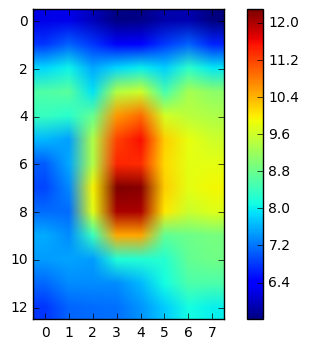
\includegraphics[width=\textwidth]{img/sample2_heatmap.png}
\caption{Heat-map for 5P\label{fig:sample2_hm}}
\end{subfigure}
\begin{subfigure}[b]{0.3\textwidth}
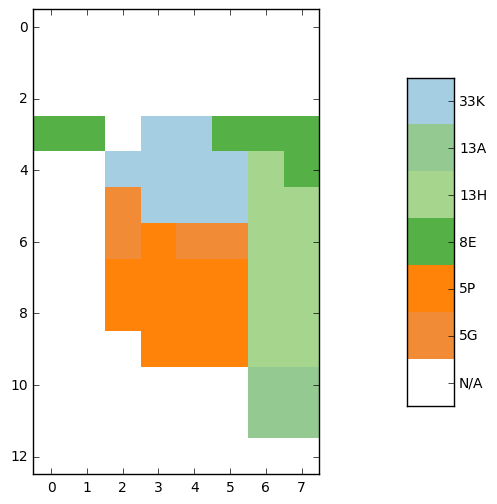
\includegraphics[width=\textwidth]{img/sample2_labels.png}
\caption{Label-map for 5P\label{fig:sample2_lab}}
\end{subfigure}

\begin{subfigure}[b]{0.3\textwidth}
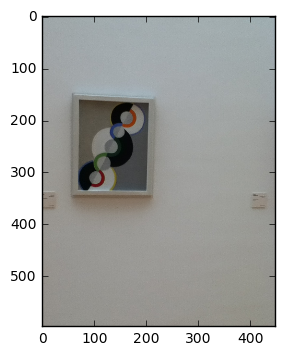
\includegraphics[width=\textwidth]{img/sample3_30P-0976.png}
\caption{Image with label 30P\label{fig:sample3_id}}
\end{subfigure}
\begin{subfigure}[b]{0.3\textwidth}
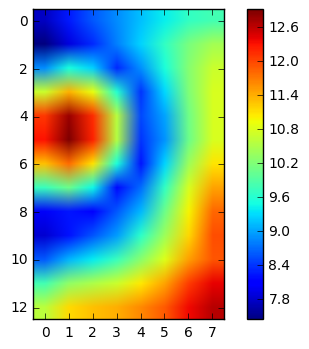
\includegraphics[width=\textwidth]{img/sample3_heatmap.png}
\caption{Heat-map for 30P\label{fig:sample3_hm}}
\end{subfigure}
\begin{subfigure}[b]{0.3\textwidth}
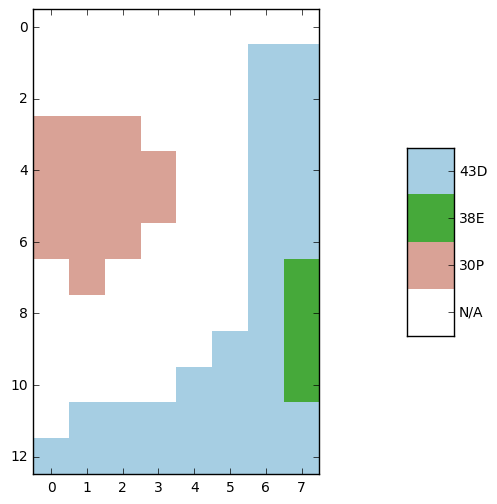
\includegraphics[width=\textwidth]{img/sample3_labels.png}
\caption{Label-map for 30P\label{fig:sample3_lab}}
\end{subfigure}
\caption{Sample images (scaled to a smaller side of 448 pixels)
along with the heat-map of maximal activation values
at each location when a fine-tuned ResNet-152 is applied to the image in a
strided manner, as well as the labels of all maximal activations that are
greater than the mean maximal activation\label{fig:heatmaps}}
\end{figure}

Previous approaches in image retrieval
~\cite{gordo_end--end_2017,salvador_faster_2016,tolias_particular_2015}
usually deal with regions of interest in one way or another.
The idea is that in most cases, only certain parts of each image can
be useful for comparison with other images. In addition to this,
cropping images at their regions of interest can help with differences
in scale of the images to compare: if a building is visible only in a small
part of an image, cropping the image at that part and then re-scaling
the part should set the building at a normalized scale.

However, in instance search with museum datasets, it is not obvious
where the regions of interest should be: most images represent an entire
painting or parts of it and only some may contain the painting as part
of the image with a wall in the background. This means for most images,
the ground-truth region of interest is simply the entire image, and some
may have a ground-truth region of interest which is almost the entire image,
excluding only a small part of the background.

On the other hand, a network fine-tuned on classification on such a dataset
should be able to easily identify the region containing the painting, since
the background wall is contained in almost all classes, which means it is a
particularly bad indicator of the class. Thus, if the network is applied in
a strided manner across an image, it should produce low maximal activations
in parts containing big sections of background wall. This idea of using a
network fine-tuned on classification as a predictor of regions of interest
has already been investigated by Oquab et al.~\cite{oquab_is_2015}. They
show that a CNN can predict approximate locations of objects using a
multi-scale sliding window training.

Figure~\ref{fig:heatmaps} shows images, along with the heat map
representing the maximal activation of a fine-tuned ResNet-152 at
each coordinate, when the network is applied in a strided manner
across the input image. The fine-tuning was carried out as described in
Section~\ref{sec:finetuning}.
From this image, we can see that the highest maximal
activations of the network usually occur at the location of the object.
This is true even if the object is not correctly classified by some of
the highest activations as can be seen in images
~\ref{fig:sample2_id}~-~\ref{fig:sample2_lab}.

In the images
~\ref{fig:sample3_id}~-~\ref{fig:sample3_lab}, it seems like many
high maximal activations occur specifically in the background area.
However, the corresponding label-map shows that these areas correspond
to the labels 38E and 43D. Both of these labels are pieces of art which
consist mostly of the background wall. In this sense, it is not
entirely wrong to consider \emph{wall-only} patches of the image as
instances of these pieces of art. This simply means that the image
consists of two separate regions of interest: one region with the painting
(label 30P) and one region containing only the wall (labels 38E/43D).

From these observations, we can confirm the assumption that the
maximal activations of a fine-tuned network are a good indicator of
the location of an object, or a combination of different objects.
Using this assumption, there is no need
for a procedure to annotate regions of interest, as employed by most
state-of-the-art image retrieval approaches
~\cite{gordo_deep_2016,tolias_particular_2015,radenovic_cnn_2016}.

On the other hand, using datasets developed for image retrieval,
such as Paris6k or Oxford5k~\cite{philbin_lost_2008,philbin_object_2007},
this assumption cannot be applied, since the dataset is not clean
enough for a network fine-tuned on classification to be a good indicator
of location of the query objects.

\subsection{Incorrectly identified images}\label{sec:incorrectimages}
\begin{figure}
\centering
\begin{subfigure}{\textwidth}
\begin{tabular}{!{\vrule width 2pt}c!{\color{green}\vrule width 2pt}c!{\color{green}\vrule width 2pt}*{5}{c}}
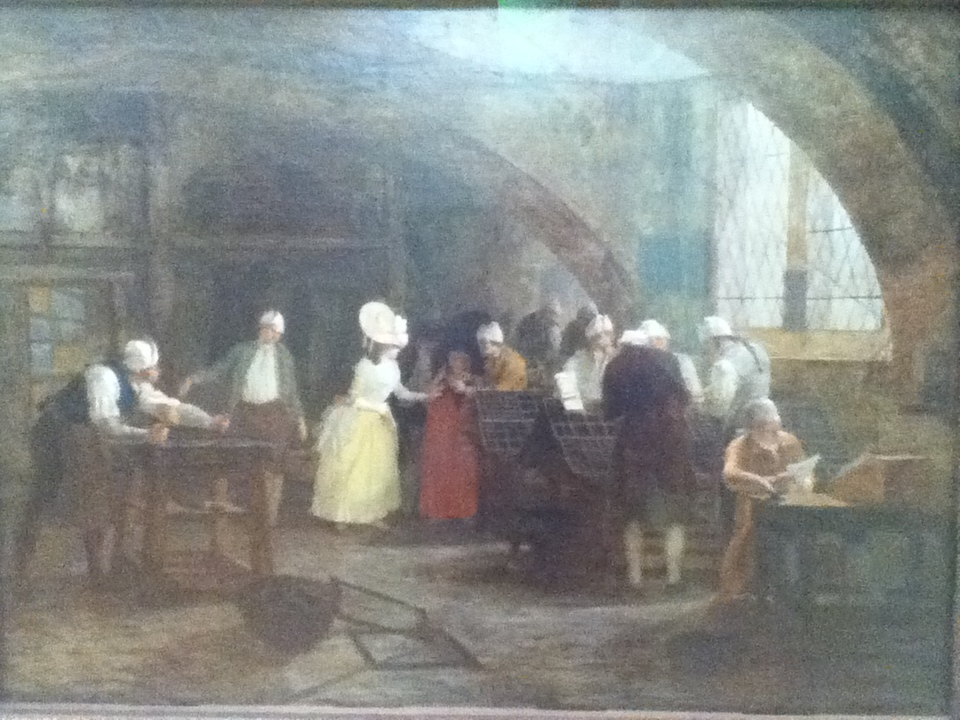
\includegraphics[width=0.12\textwidth]{img/11J-0521.JPG} &
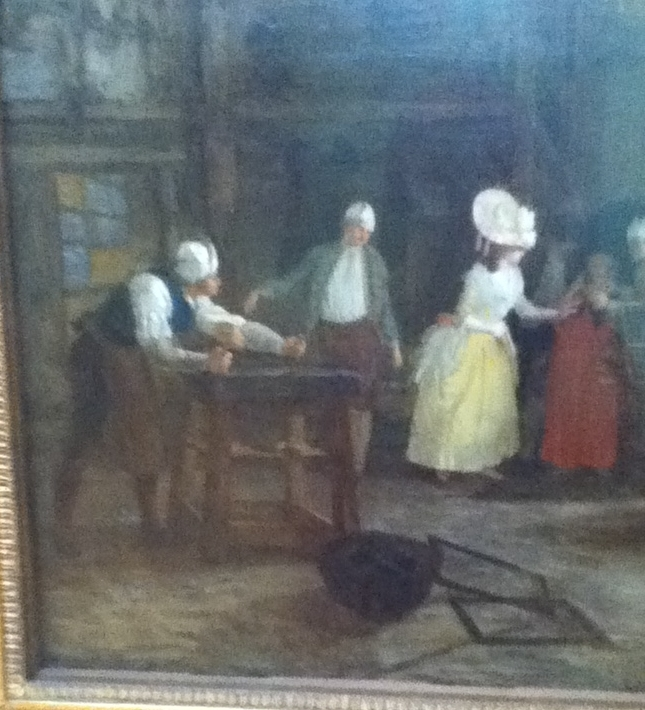
\includegraphics[width=0.12\textwidth]{img/11J-4.JPG} &
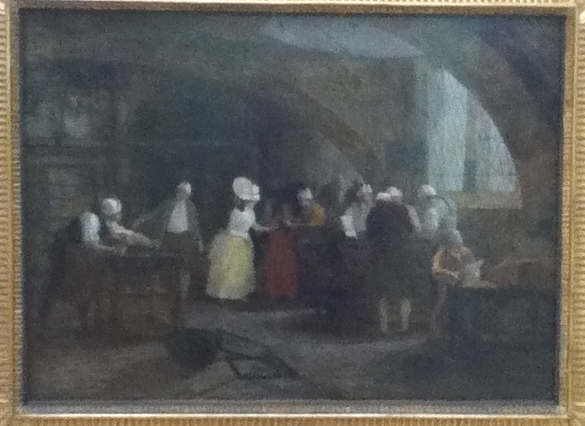
\includegraphics[width=0.12\textwidth]{img/11J-1.JPG} &
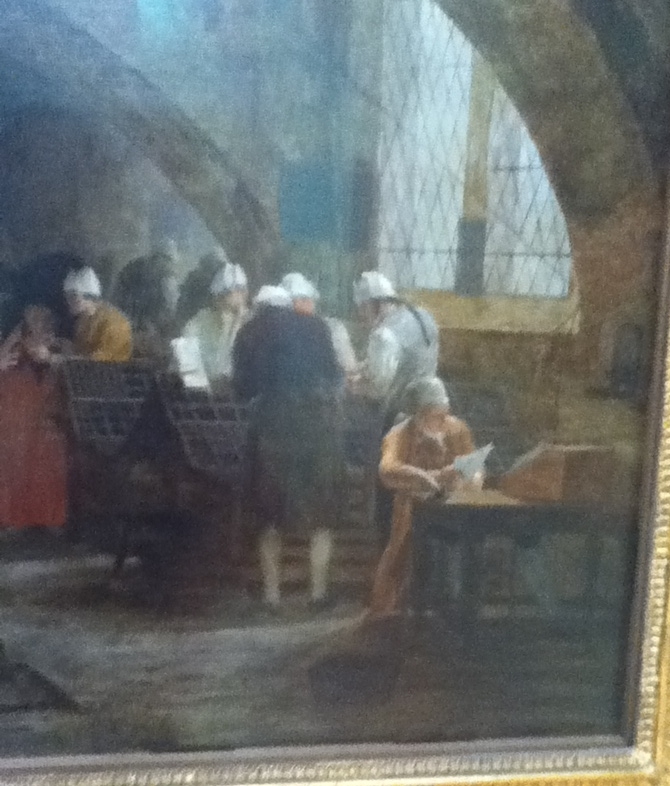
\includegraphics[width=0.12\textwidth]{img/11J-2.JPG} &
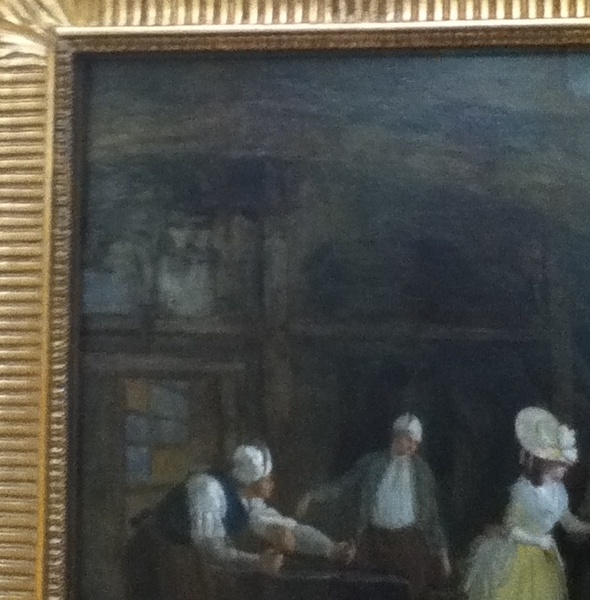
\includegraphics[width=0.12\textwidth]{img/11J-3.JPG} &
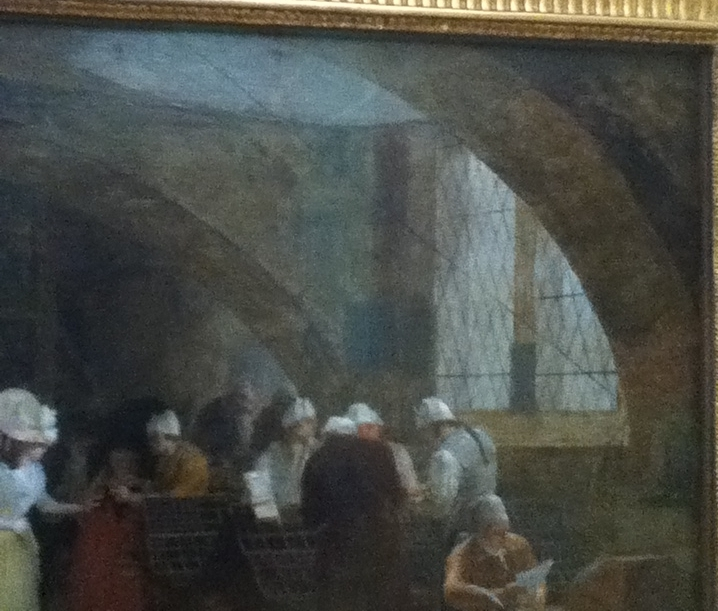
\includegraphics[width=0.12\textwidth]{img/11J-0.JPG} \\
\end{tabular}
\caption{Correctly identified query
along with the best match and all other possible reference images.\newline
Average precision Gordo et al.~\cite{gordo_deep_2016} (ResNet-50, multi-res): 1.0,
fine-tuned ResNet-152: 1.0
\label{fig:correct11J}}
\end{subfigure}

\begin{subfigure}{\textwidth}
\begin{tabular}{!{\vrule width 2pt}c!{\color{green}\vrule width 2pt}c!{\color{green}\vrule width 2pt}*{5}{c}}
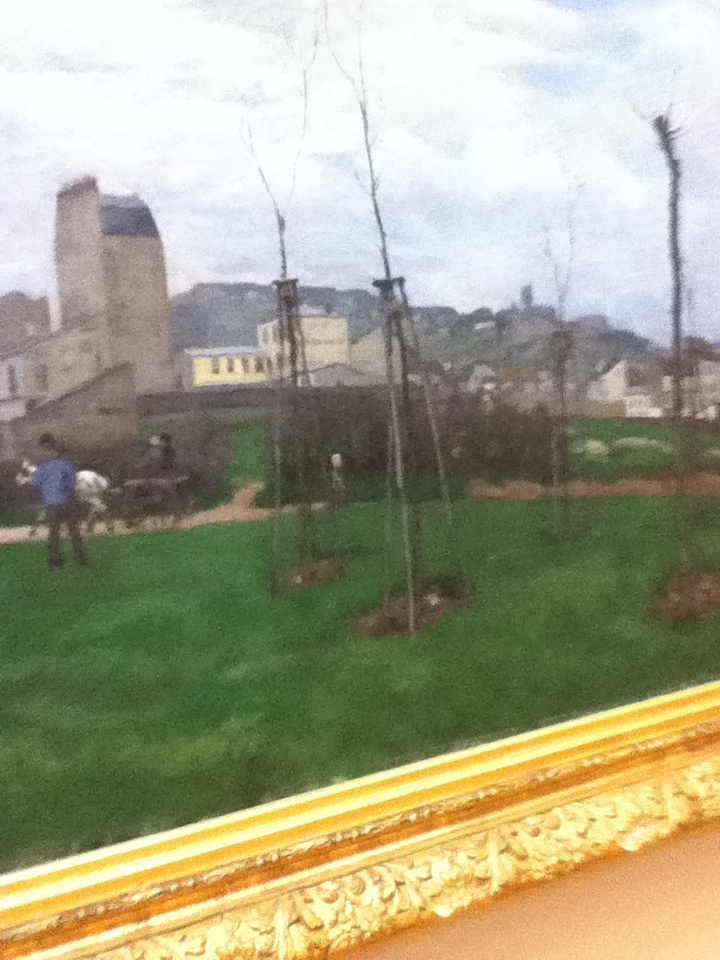
\includegraphics[width=0.12\textwidth]{img/23D-0740.JPG} &
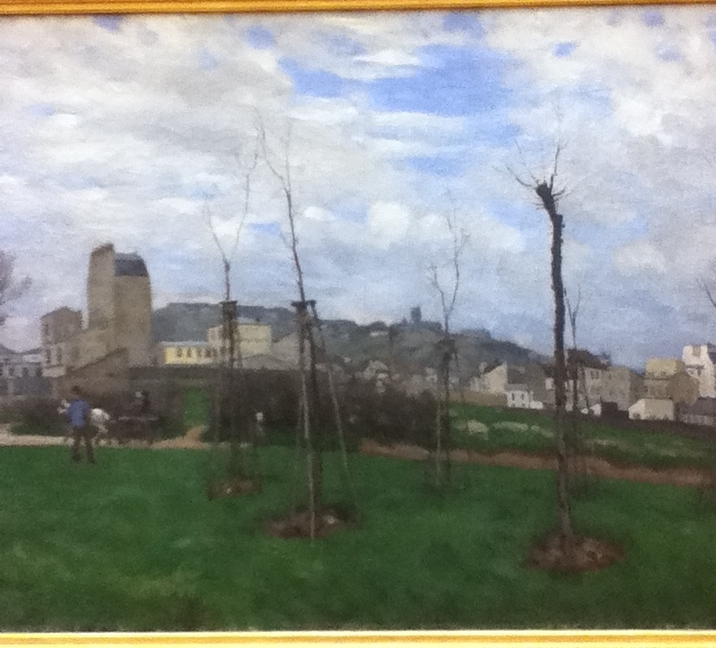
\includegraphics[width=0.12\textwidth]{img/23D-2.JPG} &
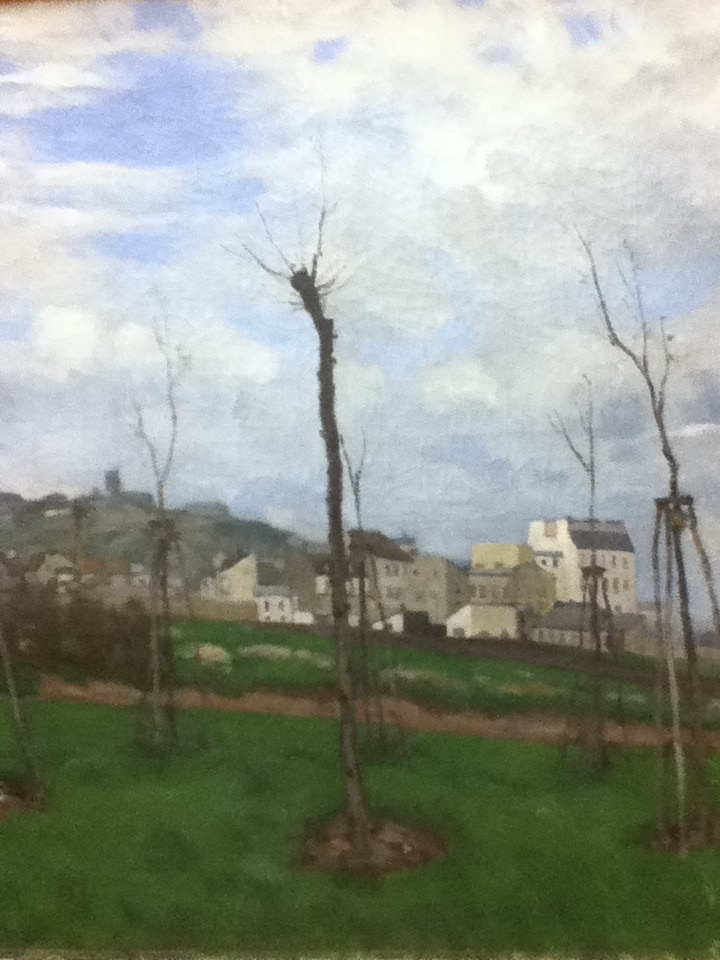
\includegraphics[width=0.12\textwidth]{img/23D-1.JPG} &
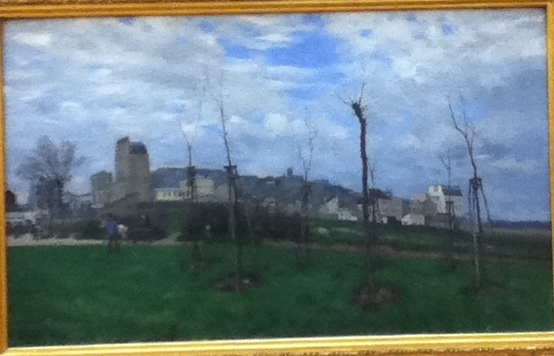
\includegraphics[width=0.12\textwidth]{img/23D-0.JPG} &
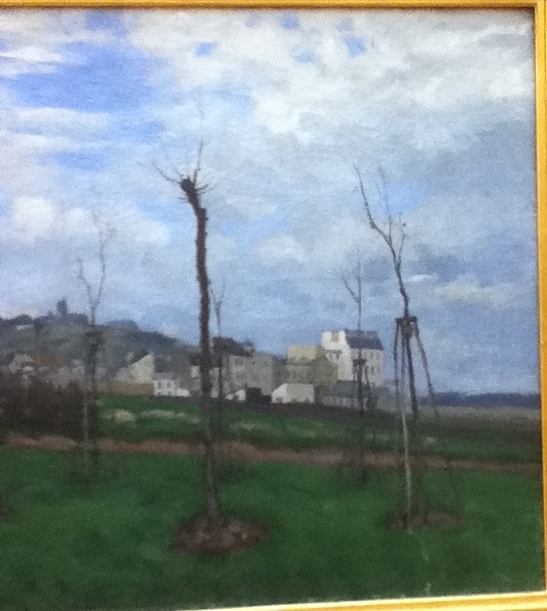
\includegraphics[width=0.12\textwidth]{img/23D-3.JPG} &
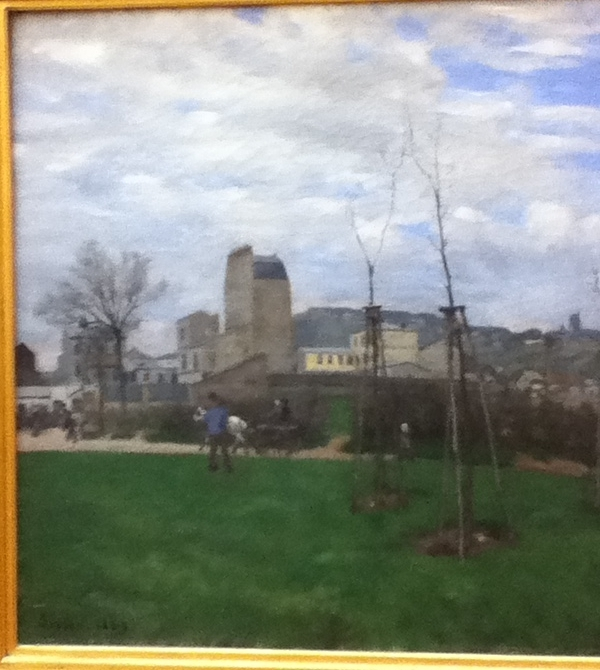
\includegraphics[width=0.12\textwidth]{img/23D-4.JPG} &
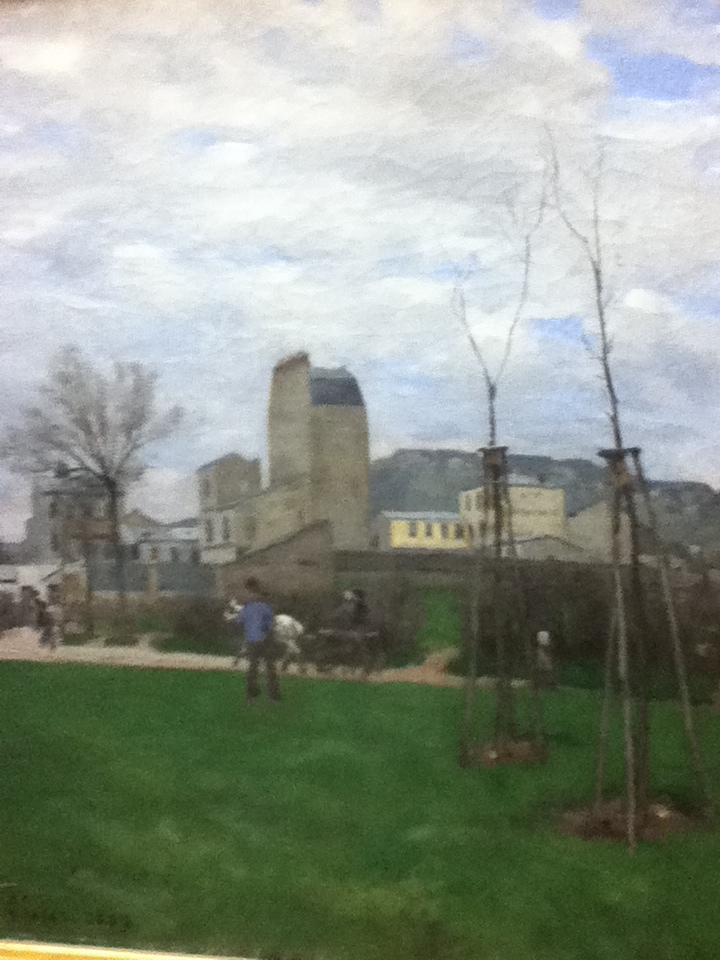
\includegraphics[width=0.12\textwidth]{img/23D-5.JPG} \\
\end{tabular}
\caption{Correctly identified query,
along with the best match and all other possible reference images.\newline
Average precision Gordo et al.~\cite{gordo_deep_2016} (ResNet-50, multi-res): 1.0,
fine-tuned ResNet-152: 1.0
\label{fig:correct23D}}
\end{subfigure}

\begin{subfigure}{\textwidth}
\begin{tabular}{!{\vrule width 2pt}c!{\color{red}\vrule width 2pt}c!{\color{red}\vrule width 2pt}*{5}{c}}
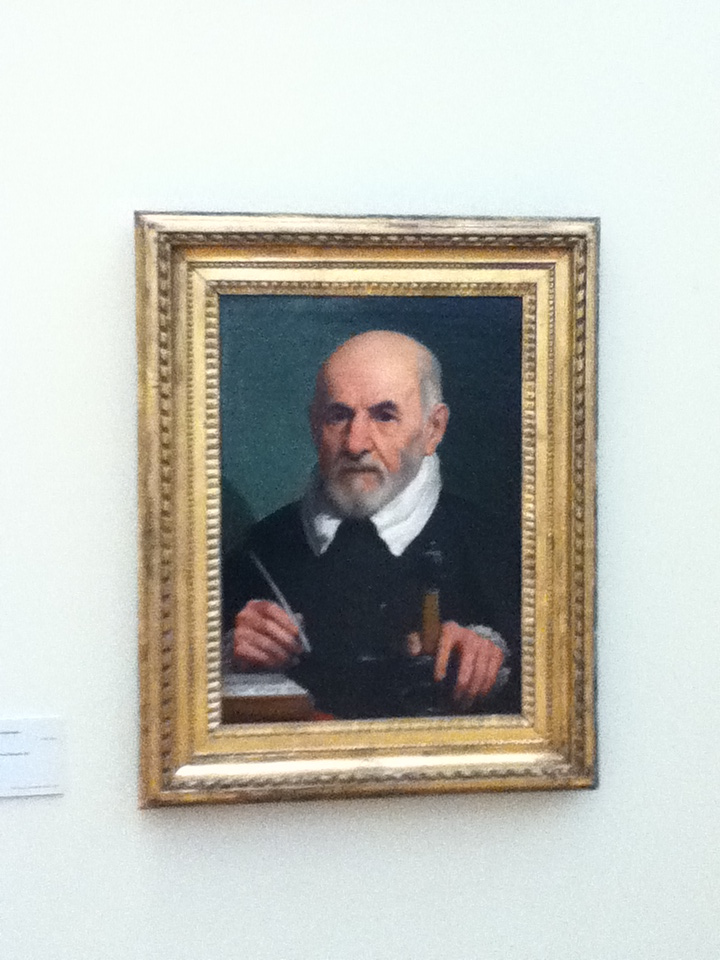
\includegraphics[width=0.12\textwidth]{img/1C-0454.JPG} &
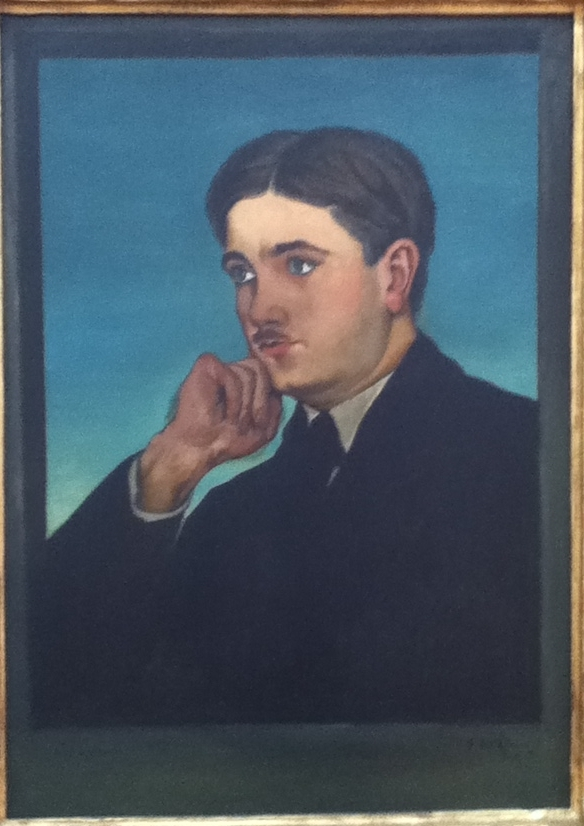
\includegraphics[width=0.12\textwidth]{img/1C-0454-36A-1.JPG} &
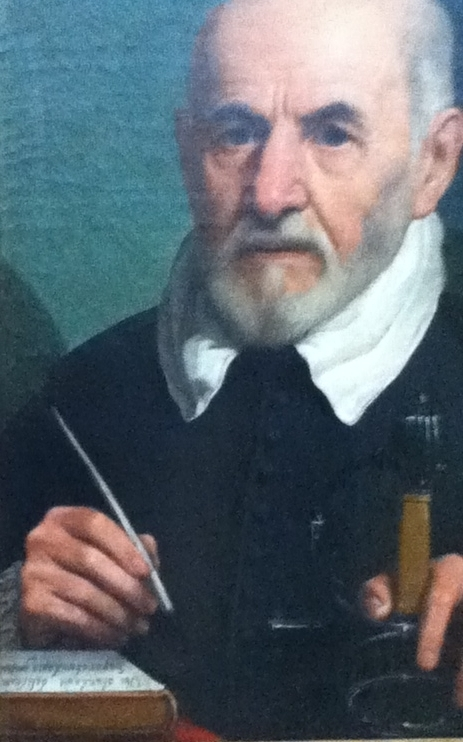
\includegraphics[width=0.12\textwidth]{img/1C-0.JPG} &
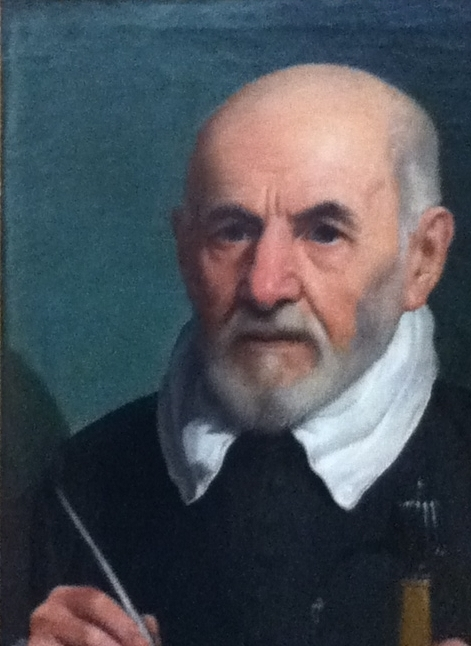
\includegraphics[width=0.12\textwidth]{img/1C-1.JPG} &
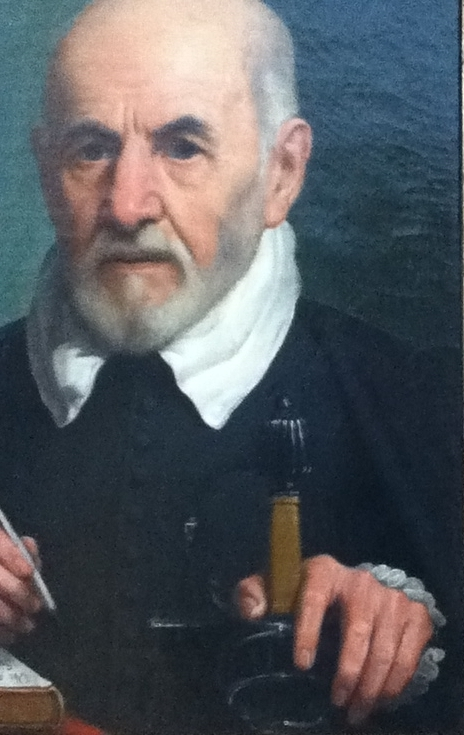
\includegraphics[width=0.12\textwidth]{img/1C-2.JPG} &
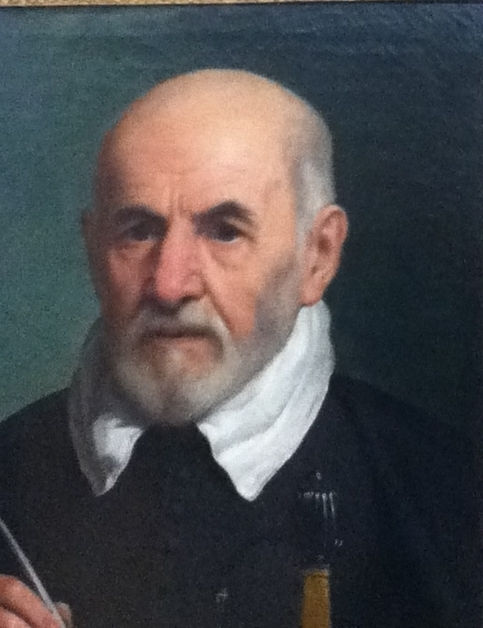
\includegraphics[width=0.12\textwidth]{img/1C-3.JPG} &
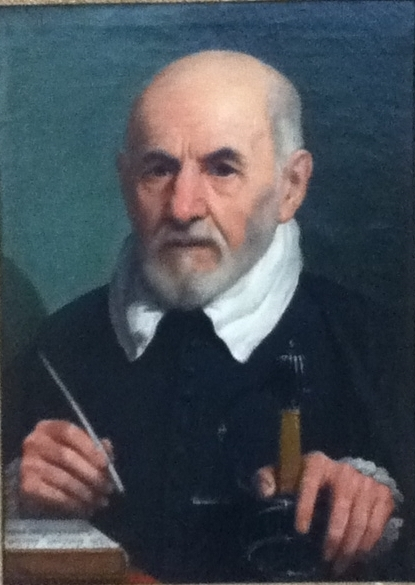
\includegraphics[width=0.12\textwidth]{img/1C-4.JPG} \\
\end{tabular}
\caption{Incorrectly identified query
along with the best match and all possible reference images.\newline
Average precision Gordo et al.~\cite{gordo_deep_2016} (ResNet-50, multi-res): 0.113,
fine-tuned ResNet-152: 0.014
\label{fig:incorrect1C}}
\end{subfigure}

\begin{subfigure}{\textwidth}
\begin{tabular}{!{\vrule width 2pt}c!{\color{red}\vrule width 2pt}c!{\color{red}\vrule width 2pt}*{5}{c}}
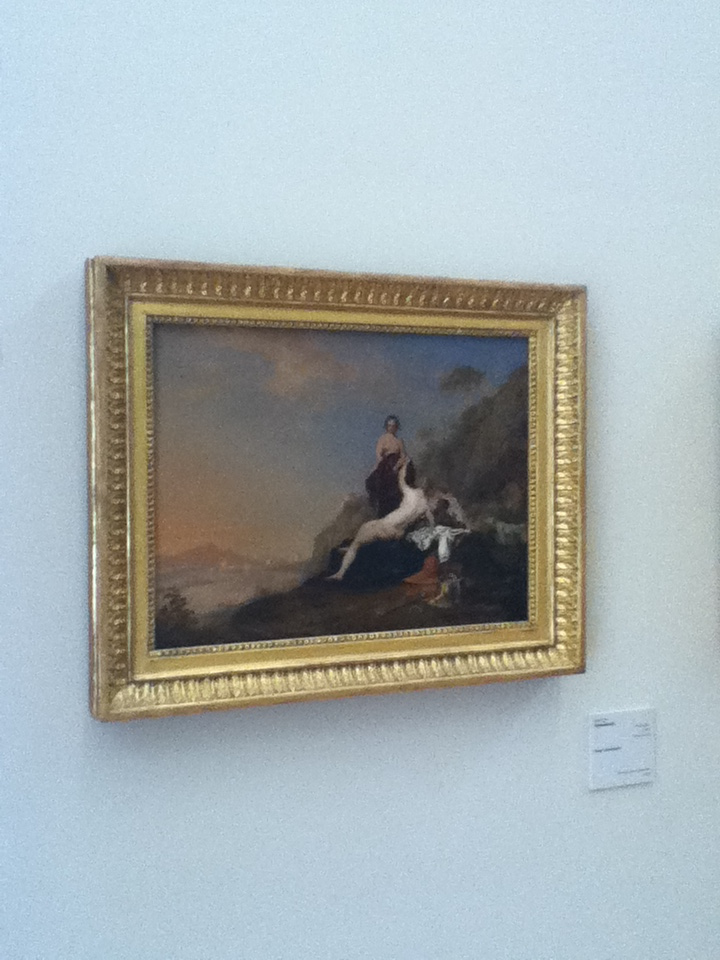
\includegraphics[width=0.12\textwidth]{img/5B-0506.JPG} &
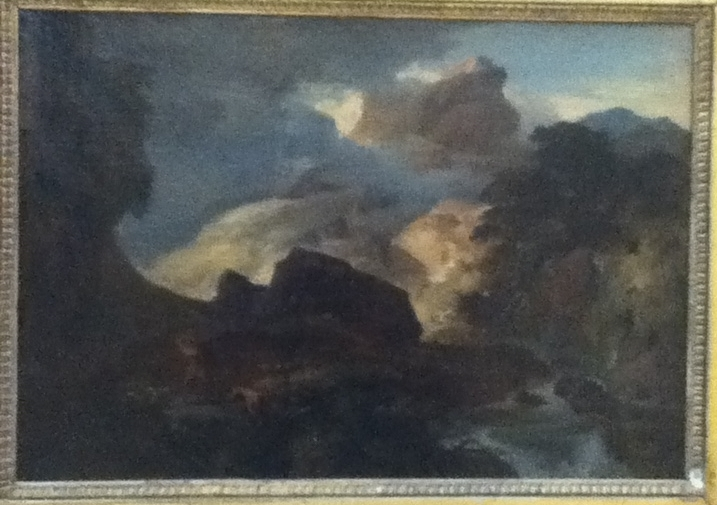
\includegraphics[width=0.12\textwidth]{img/5B-0506-16M-0.JPG} &
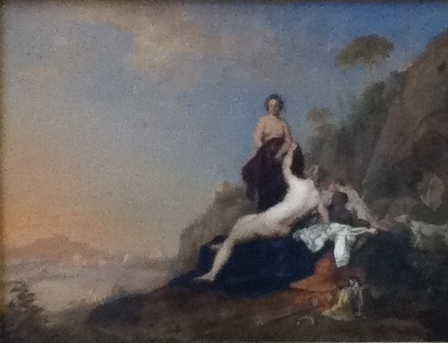
\includegraphics[width=0.12\textwidth]{img/5B-0.JPG} &
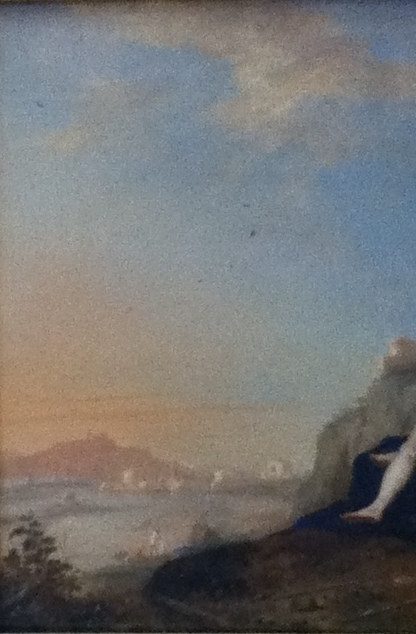
\includegraphics[width=0.12\textwidth]{img/5B-1.JPG} &
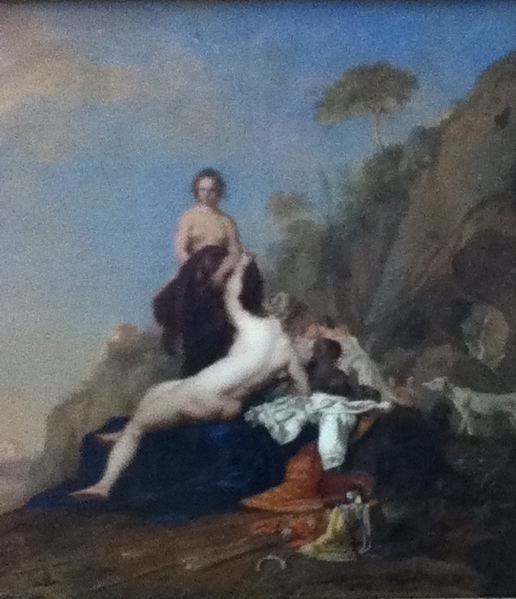
\includegraphics[width=0.12\textwidth]{img/5B-2.JPG} &
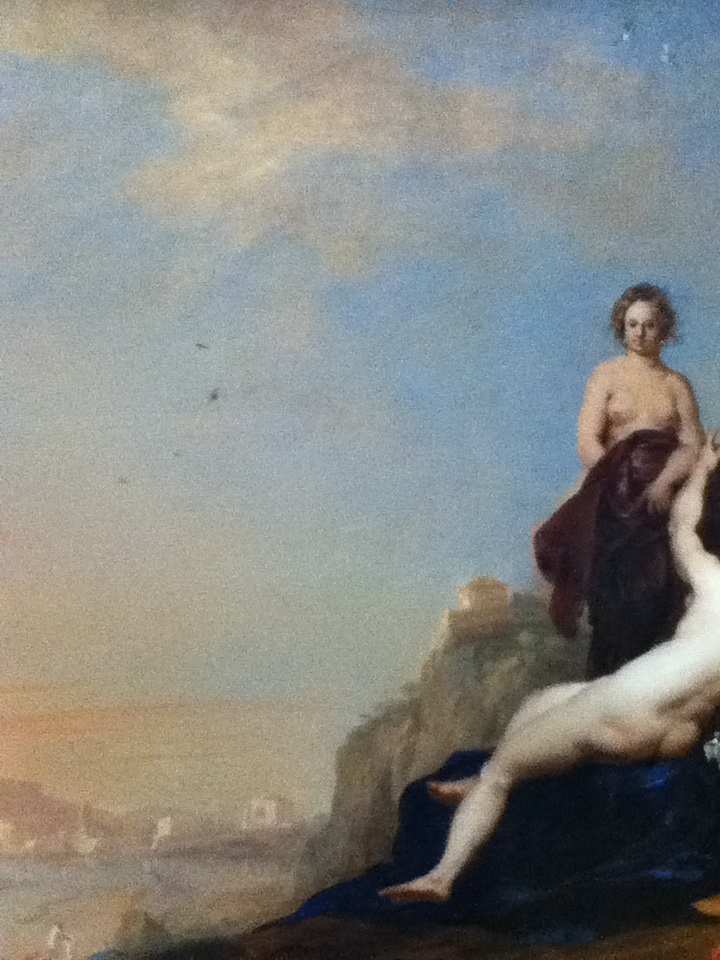
\includegraphics[width=0.12\textwidth]{img/5B-3.JPG} &
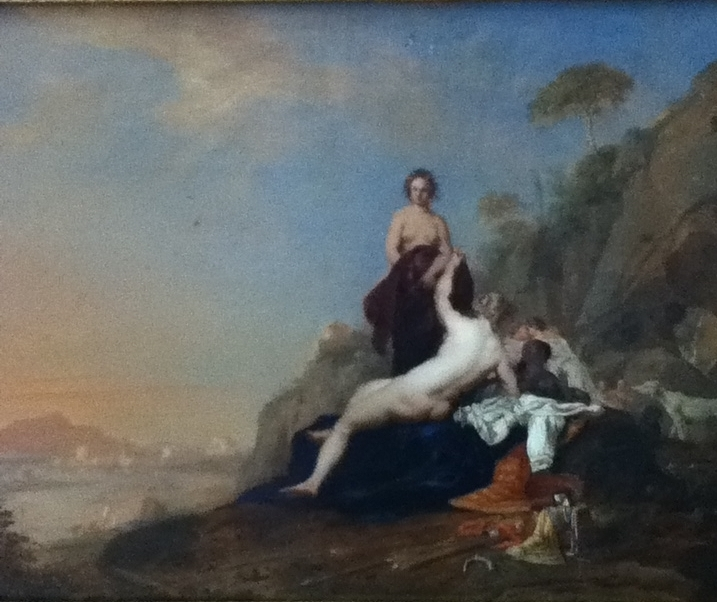
\includegraphics[width=0.12\textwidth]{img/5B-4.JPG} \\
\end{tabular}
\caption{Incorrectly identified query
along with the best match and all possible reference images.\newline
Average precision Gordo et al.~\cite{gordo_deep_2016} (ResNet-50, multi-res): 0.013,
fine-tuned ResNet-152: 0.002
\label{fig:incorrect5B}}
\end{subfigure}

\begin{subfigure}{\textwidth}
\begin{tabular}{!{\vrule width 2pt}c!{\color{red}\vrule width 2pt}c!{\color{red}\vrule width 2pt}*{5}{c}}
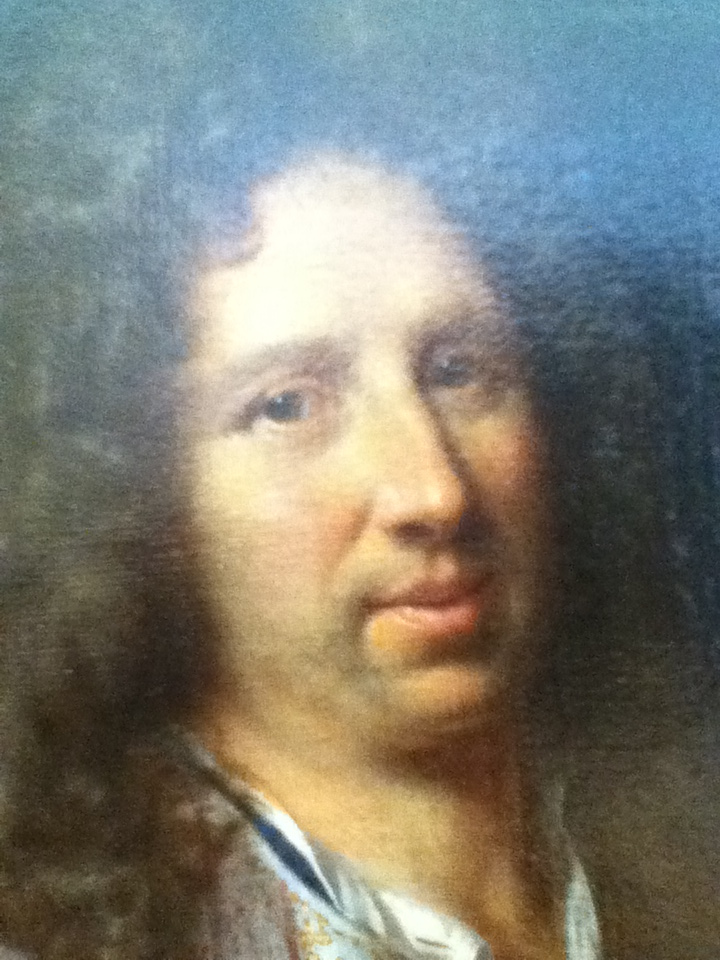
\includegraphics[width=0.12\textwidth]{img/11C-0351.JPG} &
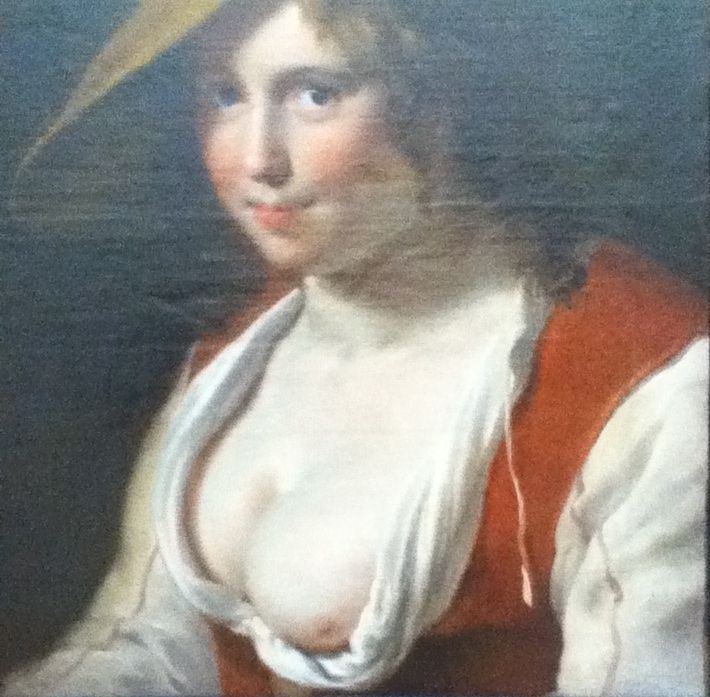
\includegraphics[width=0.12\textwidth]{img/11C-0351-6D-0.JPG} &
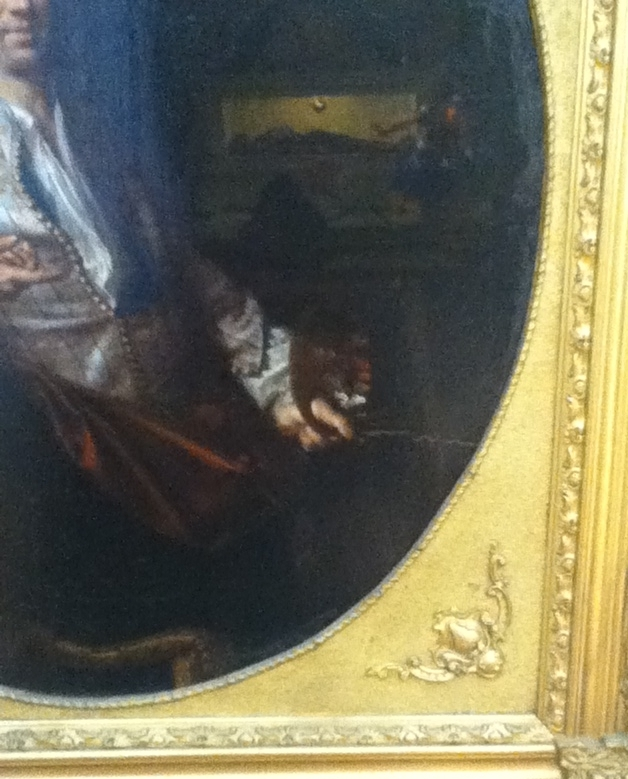
\includegraphics[width=0.12\textwidth]{img/11C-0.JPG} &
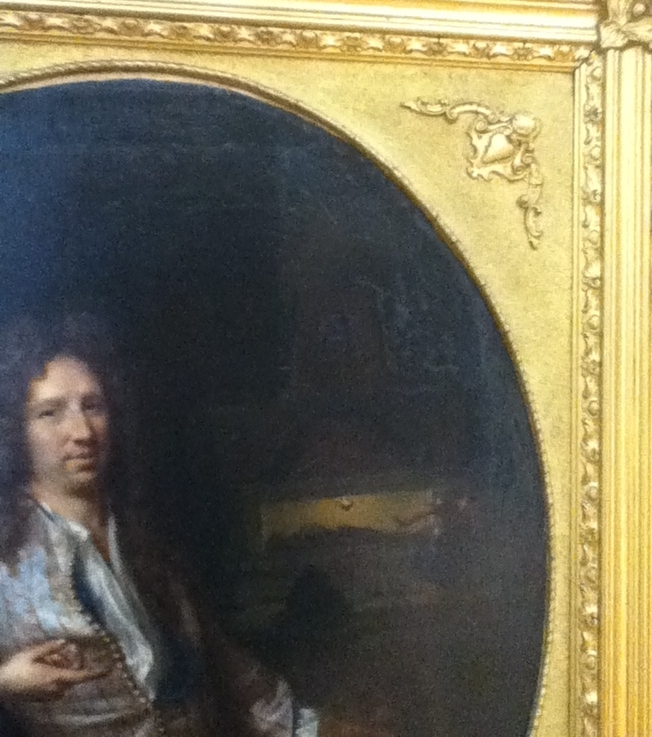
\includegraphics[width=0.12\textwidth]{img/11C-1.JPG} &
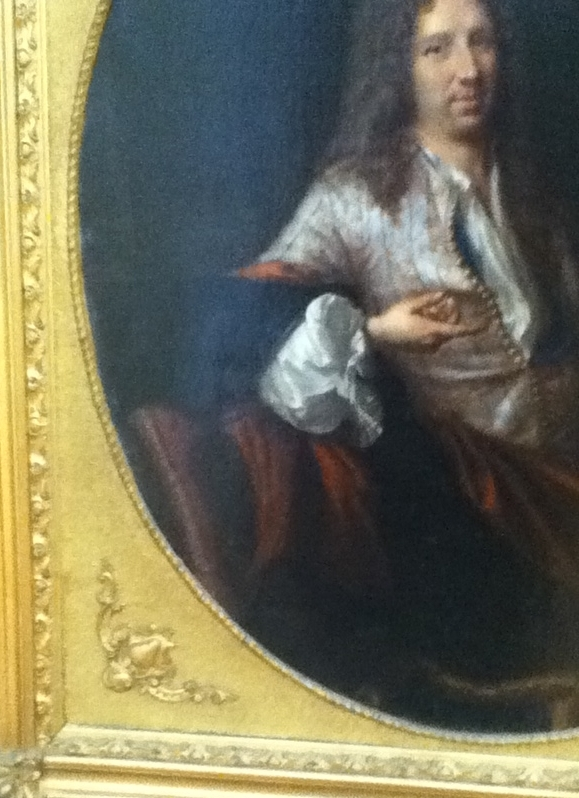
\includegraphics[width=0.12\textwidth]{img/11C-2.JPG} &
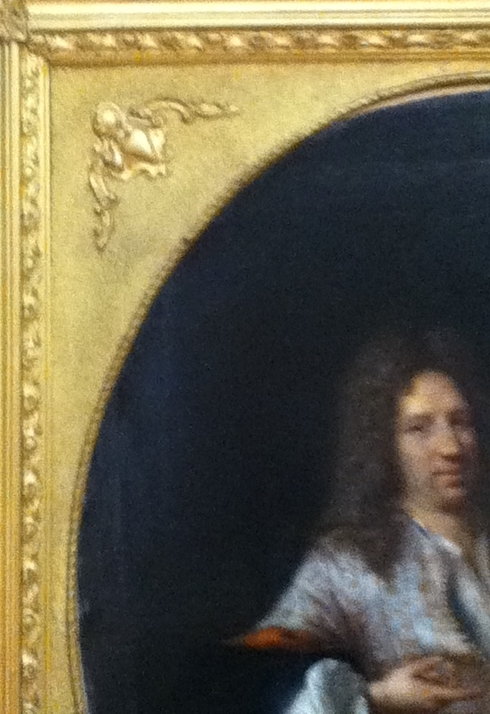
\includegraphics[width=0.12\textwidth]{img/11C-3.JPG} &
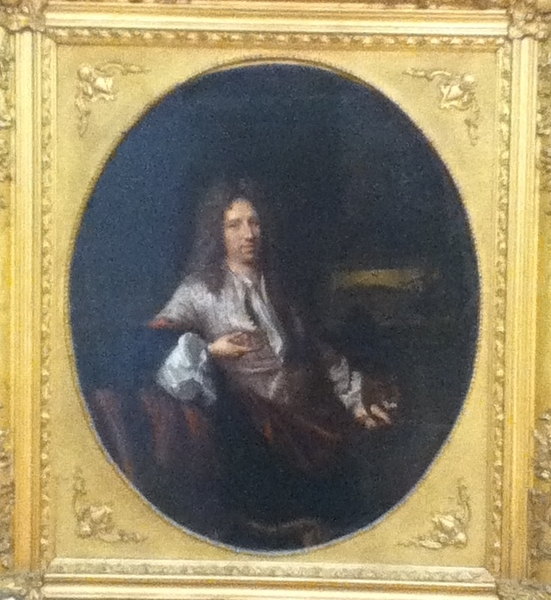
\includegraphics[width=0.12\textwidth]{img/11C-4.JPG} \\
\end{tabular}
\caption{Incorrectly identified query
along with the best match and all possible reference images.\newline
Average precision Gordo et al.~\cite{gordo_deep_2016} (ResNet-50, multi-res): 0.004,
fine-tuned ResNet-152: 0.004
\label{fig:incorrect11C}}
\end{subfigure}
\caption{Sample images that were correctly and incorrectly identified
by a fine-tuned ResNet-152, as well as the modified ResNet-50 published by
Gordo et al.~\cite{gordo_deep_2016} using images at multiple resolutions. For each image,
the query image is shown at the very left, the best match of the ResNet-50 is shown next to it with green bars indicating a correct match, red bars indicating a wrong match, and all possible correct reference
images are shown to the right of the query. The caption contains the
associated average precision values.
Note that this figure is best viewed in color.
\label{fig:incorrectimg}}
\end{figure}

Figure~\ref{fig:incorrectimg}
shows typical images that were correctly identified versus images that
were incorrectly identified, by a fine-tuned network as well as the network
published by Gordo et al.~\cite{gordo_deep_2016}, along with the average
precision for the respective queries.

From these results, we see that the networks struggle with images at
very different scales, achieving very low average precision,
while images with similar scales are usually perfectly matched.

% TODO more detail
Combining both of the properties identified in this section, we
propose a novel approach to learn a strong descriptor for instance
search in the next section.

\section{Proposed instance search architecture}\label{sec:proposed}
The proposed approach is based on multiple steps as described in the
following sections.

\subsection{Fine-tuning on classification using an FCN}\label{sec:fcnfinetune}
As shown in Section~\ref{sec:analysisprev}, a fine-tuned CNN is already
a good indicator of the location of an object in our datasets.
Additionally, it seems like scale is a particularly important factor.

Thus, the idea is to start by fine-tuning a network with images
at different scales. This can be achieved by using a fully
convolutional network (FCN), as introduced by
Long et al.~\cite{long_fully_2015}.

In an FCN, the final fully connected layers
of a network are replaced by convolutional layers having a kernel
which fits the entire domain of the output of the previous layer.
This type of convolution is equivalent to a fully connected layer,
but allows inputs (and outputs) of any size.
The effect is that the network can be applied in one pass to an
arbitrarily sized image. The output then represents the activations
of the network as if it was applied in a strided manner across the image.
The stride of a full network depends on the architecture and is 32
pixels for the architectures used here: AlexNet and ResNet.

Once an FCN is applied to the image, the loss
is calculated by averaging the cross-entropy loss across all locations
and outputs.
The final loss is then obtained by passing images at different scales
through the FCN and averaging across all cross-entropy losses of all
outputs and scales. Note that we assume that most of the images contain
almost exclusively the object of interest. If this is not the case, many
patches in the sliding window would be mis-labeled.

Equation~\ref{eq:fcnloss} shows the loss for a
single image. $S$ represents the number of scales at which the image
is passed through the network.
$H_s$ and $W_s$ represent the height and width of the feature
map respectively, given the scale $s$ of the input image.
$\mathit{CE}^{h,w}$ represents the cross-entropy loss applied
at spatial location $(h,w)$ in the full feature map. It is applied
for each prediction $y^{h,w}$ of the network and the constant true label
$\hat{y}$.

\begin{equation}\label{eq:fcnloss}
\mathcal{L} = \frac{1}{S} \sum_{s=1}^S \frac{1}{H_s*W_s}
\sum_{h=1}^{H_s} \sum_{w=1}^{W_s} \mathit{CE}^{h,w}
\end{equation}

Additionally, we can see from Equation~\ref{eq:fcnloss} that we choose
to give each scale of the image the same weight in the loss. This
attenuates the effect of large scales with many predictions (high
values for $H_s$ and $W_s$).

Finally, this loss can only be applied to one image at a time because
the images are passed to the network at their true
aspect ratio, which means the loss for different images may have different
values for the heights and widths of the feature maps $H_s$ and $W_s$.

In order to normalize the sizes of the features present in the images,
all images are scaled to have the same
number of pixels in the smaller side. Note that for large aspect
ratios and large scales of the smaller side,
the memory consumption of training can be high for single images
having a very large aspect ratio. To limit this spike in memory
consumption, the aspect ratios are limited by introducing uniform
random noise on the smaller side of images with high aspect ratios.

In our experiments, we use a maximal aspect ratio of $2.0$ and images
at two scales of $448$ and $224$ pixels for the smaller side. We found
that the AlexNet architecture did not have good convergence behavior.
This is most likely due to the worse generalization property of AlexNet
as compared to ResNet and the large number of patches in an image with
smaller side $448$. Thus, for AlexNet we used scales of $384$ and $224$ instead.

\subsubsection{Gradient descent using micro-batches}
Since only a single image is passed to the network at a time, the
stochastic gradient descent algorithm used to optimize the parameters
of the model does not converge, as a single image is not representative
of the dataset as a whole and does not form a large enough mini-batch.

Instead, we form a mini-batch by accumulating gradients from many
\emph{micro-batches}, each of which is made up of only a single image.
This allows to form a mini-batch of any size to obtain stable convergence
in stochastic gradient descent.

However, using a micro-batch formed of a single image represents an issue
with the ResNet architecture: as described in Section~\ref{sec:verydeepCNNs},
this model uses batch-norm layers~\cite{ioffe_batch_2015}.
When training a model, this layer keeps a running
mean and variance, which approximates the true mean and variance of the
dataset and which is applied during testing. With a micro-batch size
of 1, this running mean and variance cannot be inferred correctly,
which leads to very poor convergence behavior of the model.
Instead, we pre-train the model on the new
dataset as described in Section~\ref{sec:finetuning} in order to obtain
a correct estimate of the running mean and variance. Then, we preset the
network with the parameters of this fine-tuned network when training the
FCN as described above.

\subsection{Descriptor extraction network}
\begin{figure}
\begin{subfigure}{\textwidth}
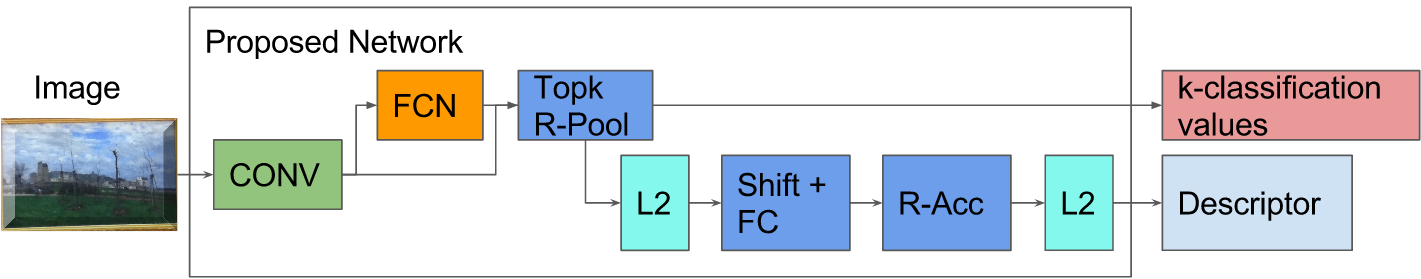
\includegraphics[width=\textwidth]{img/contrib_deploy.png}
\caption{Proposed architecture for instance search, at deploy time
\label{fig:contribdeploy}}
\end{subfigure}

\begin{subfigure}{\textwidth}
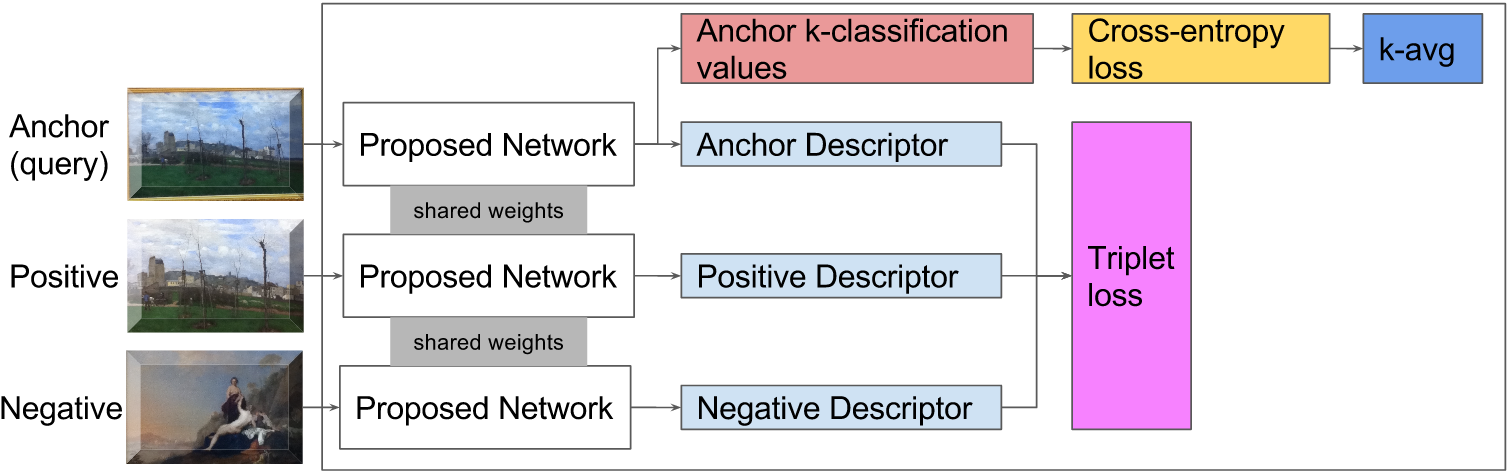
\includegraphics[width=\textwidth]{img/contrib_train.png}
\caption{Proposed architecture for instance search, at training time
\label{fig:contribtrain}}
\end{subfigure}
\caption{Proposed architecture for instance search, based on a FCN
~\cite{long_fully_2015} for region proposals. The descriptor extraction
for each region is similar to the state-of-the-art architecture
shown in Figures~\ref{fig:gordo_deploy}~and~\ref{fig:gordo_train}
\label{fig:contrib}}
\end{figure}

The second step of the proposed approach relies on the FCN, trained
as described in the first step in Section~\ref{sec:fcnfinetune}.

Figure~\ref{fig:contrib} illustrates the proposed architecture.
To obtain a descriptor, we first apply the convolutional layers of
a previous architecture, such as AlexNet or ResNet. We then obtain all
classification outputs at all locations using the pre-trained FCN.
We only consider the maximal activation at all locations.
The locations with the top $k$ maximal activations will form the descriptor.
Here, we can see that we only need an approximation of the location of
an object since the descriptor is composed of convolutional activations with a
receptive field as large as the receptive field of the whole network: usually
a patch of more than $224 \times 224$. Hence, we only need to locate objects
in this large patch, which can be achieved by an FCN as discussed by Oquab
et al.~\cite{oquab_is_2015}, and described in Section~\ref{sec:fcnfinetune}.

For each of the top $k$ locations, we closely follow the architecture
shown in
Figure~\ref{fig:gordo_deploy}. The convolutional features are
reduced by a $\|\cdot\|_2$-normalization, then a shifting and fully connected
layer. Finally, all descriptors from the $k$ locations are
sum-aggregated and $\|\cdot\|_2$-normalized again.

When training, the network is applied to a triplet of images.
These triplets are chosen as described in Section~\ref{sec:simplifiedsiam}
for the simplified Siamese architecture.

Additionally, we regularize the triplet loss by a cross-entropy loss
to make sure that the $k$ locations with highest
maximal activations are correctly classified. This loss is averaged over
the $k$ locations.

Equation~\ref{eq:proposedloss} shows the full loss as used in our
experiments to train the proposed model, for a $N$ images. In this
equation, $(h_l, w_l)$ represents the spatial coordinates of the $l$-th
region of highest maximal activation in the feature map produced by
the FCN.

\begin{equation}\label{eq:proposedloss}
\mathcal{L} = \sum_{i=1}^N \left( \max(0, x^a_i x^n_i - x^a_i x^p_i + m) +
\alpha \frac{1}{N} \frac{1}{k} \sum_{l=1}^k \mathit{CE}_i^{h_l,w_l} \right)
\end{equation}

In our experiments, we choose the number of regions with highest maximal
activation to be $k=6$ and the regularization hyper-parameter $\alpha=1.0$.
The margin of the triplet loss is $m=0.1$ as described in
Section~\ref{sec:simplifiedsiam}.

The results obtained by the proposed approach are listed in Table~\ref{tab:results} in chapter~\ref{chap:results}.

\subsection{Advantages and limitations}
As shown in Section~\ref{sec:analysisprev}, this approach
allows the network to decide which region of interest is
best suited for classification and ultimately which regions
are best suited for comparison with other images.

Another advantage is that this approach does not require
any annotation of the images with regions of interest,
which can be a long, manual or automatic process, as evident
from the cleaning process used by Gordo et al.~\cite{gordo_end--end_2017}.

Finally, an important property of the descriptor is that it
heavily relies on the classification
capabilities of the network. This means the descriptor is
mostly meaningless for a different dataset and needs
to be learned for each dataset. This can be an advantage,
since the descriptor can be better suited to a particular
dataset and the learning process does not take long, as shown
in Section~\ref{sec:perfresults}. On the other hand, this means that
the descriptor cannot be applied in a typical image retrieval
task.

Another limitation is the following: for the region descriptor extracted from
an FCN to be robust, the dataset used to fine-tune the FCN needs to be
very clean, as described in Section~\ref{sec:analysisprev}. Since there
are very few images per instance and each instance represents a class,
a classification network can easily identify a class if it consists
of one or two images representing background noise. This can render
the region descriptor meaningless, since in this case, any part of an image
which contains mostly background noise may be labeled with high confidence
as such a \emph{background noise instance}. For the region descriptor to be
meaningful, it is thus important that the training images contain only
\emph{meaningful} representations of instances and that they are
correctly labeled with respect to those instances.

\section{Augmenting image descriptors}\label{sec:improvedesc}
Up to this point, we consider each approach
as if it provides a single, strong descriptor for each image.
In information retrieval, many approaches combine descriptors,
or use augmentation techniques in order to improve the results
provided by a single descriptor.

The following sections quickly describe these approaches and
justify whether or not they may improve the results obtained
here.

\subsection{Combination of descriptors}
Many approaches in information retrieval combine multiple
descriptors in order to achieve better results
~\cite{philbin_lost_2008,jegou_accurate_2010,chum_total_2007}.
In particular,
it is common to combine SIFT descriptors~\cite{lowe_distinctive_2004}
and multi-scale Hessian interest points~\cite{mikolajczyk_scale_2004}.
However, one of the main motivations for our research is precisely to avoid
this combination by using an end-to-end approach based
on optimizing a single descriptor globally. On the other hand,
individual descriptors are usually optimized for
a specific task, such as scale-invariance or lighting invariance.
Since we want to avoid choosing
different descriptors to combine, we do not explore this approach.

\subsection{Query expansion}
Query expansion is a method of improving results by performing
multiple queries: first, the
descriptor of a query image is used as-is. Then, the descriptor
is combined with the descriptors of the top $k$ retrieved
results, by simply adding the descriptors together. This new
descriptor is used to perform a second query, which gives
the final result.

This technique was introduced by
Chum et al.~\cite{chum_total_2007} and is especially useful
when the descriptor of the query can be spatially matched
against the returned descriptors. This eliminates some of the
returned descriptors from the combined descriptor used
to perform a second query. However, as CNNs produce
global descriptors of images, this spatial matching cannot
be performed.

Furthermore, we do not expect query expansion to provide
any major improvements in our research problem, since
we expect to have very few images returned. This means
the only plausible value of $k$ would be $k=1$. However,
if the best matching descriptor of the first query already
matched, the second query cannot improve the result
and if it does not match, it is unlikely that the second
query would match. Overall, query expansion may
improve mean average precision, but it is unlikely to
improve mean precision@1.

\subsection{Database-side feature augmentation}
Another common approach to improve the performance of descriptors
in image retrieval was introduced
by Turcot and Lowe~\cite{turcot_better_2009} and
Arandjelovic and Zisserman~\cite{arandjelovic_three_2012}.

The idea is to combine the descriptors of the reference
images in order to form more robust database-side descriptors.
Every reference descriptor is replaced by a
combination of itself and the $k$ nearest neighbors.
This combination is computed as a weighted sum, weighted
by the rank of the neighbors with respect to $k$ (the
closest neighbor has the highest weight and the $k$-th
neighbor the lowest).
The neighbors can be pre-computed once all descriptors
have been computed for the reference images, by comparing
each image to all others. This can be done efficiently
in our case where descriptors can be compared to other
descriptors using a matrix multiplication.

However, it is difficult to choose the value for $k$, as
it should be low enough to not include many irrelevant
images for the descriptors, but high enough for the
technique to have an impact at all.

\subsection{Instance feature augmentation}\label{sec:ifa}
Since we have the labels of the reference images
available, we propose an approach similar to
database-side feature augmentation in order to
improve the results: each descriptor is replaced by a
combination of itself with all the descriptors of the same instance.

Just as in database-side feature augmentation, for each descriptor,
we compute a weighted average of the neighboring descriptors, with the
neighbors being all descriptors of reference images of the same instance.
For each descriptor, the average is weighted by the rank of the other
descriptors in comparison to it. Finally, the resulting descriptor
is normalized again.

The results obtained by instance feature augmentation are listed in Table~\ref{tab:results} in chapter~\ref{chap:results}, abbreviated by \emph{IFA}.

